\RequirePackage[l2tabu, orthodox]{nag}

\documentclass[11pt]{scrartcl}
\usepackage[utf8]{inputenc}
\usepackage{lmodern} 
\usepackage[sc]{mathpazo}


\usepackage{microtype}

\usepackage{hyperref}
\usepackage{graphicx}

\usepackage{mathtools}
\usepackage{amsthm}
%, amssymb, amsthm

\usepackage{booktabs}
\usepackage{todonotes}

\usepackage[msc-links]{amsrefs}
%\usepackage{biblatex}

\usepackage{tikz}


% Italics, Numbered
\theoremstyle{plain}
\newtheorem{thm}{Theorem}[section] % reset theorem numbering for each chapter

% Plain, Numbered
\theoremstyle{definition}
\newtheorem{defn}[thm]{Definition} % definition numbers are dependent on theorem numbers
\newtheorem{eg}[thm]{Example} % same for example numbers

% Italics, Not Numbered
\theoremstyle{plain}
\newtheorem*{note}{Note}
\newtheorem*{remark}{Remark}

\title{
	\textbf{Insert Title}\\ 
	{\normalsize (subtitle)}
}
\author{D. Zack Garza}
\date{\today}
\begin{document}

\maketitle

\tableofcontents

\section{Main}

\begin{thm}
All $a$'s are $b$'s. 
\end{thm}

\begin{defn}
Abcdde\cite{	hatcherAlgebraicTopologya}
\todo{Rewrite this answer $\ldots$ cd}
\end{defn}

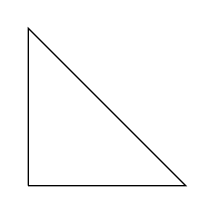
\begin{tikzpicture}
\draw (0,0) -- (0,2) -- (2,0)-- (0,0);
\end{tikzpicture}

\newpage
\section{Todo}
\listoftodos 

\bibliography{/home/zack/Notes/library.bib} 


\end{document}
